\documentclass{chi-ext}
% Please be sure that you have the dependencies (i.e., additional LaTeX packages) to compile this example.
% See http://personales.upv.es/luileito/chiext/

\copyrightinfo{
    Copyright is held by the author/owner(s).\\
        \emph{CHI'13}, April 27 -- May 2, 2013, Paris, France.\\
        ACM 978-1-XXXX-XXXX-X/XX/XX.\\
}

\title{Handwriting in the Air, Recognizing Characters on the Fly}

\numberofauthors{3}
% Notice how author names are alternately typesetted to appear ordered in 2-column format;
% i.e., the first 4 authors on the first column and the other 4 authors on the second column.
% Actually, it's up to you to strictly adhere to this author notation.
\author{
    \alignauthor{
        \textbf{Sharad Vikram}\\
            \affaddr{Computer Science Division}\\
            \affaddr{UC Berkeley}\\
            \email{sharad.vikram@berkeley.edu}
    }
    \alignauthor{
        \textbf{Lei Li}\\
            \affaddr{Computer Science Division}\\
            \affaddr{UC Berkeley}\\
            \email{leili@cs.berkeley.edu}
    }
    \alignauthor{
        \textbf{Stuart Russell}\\
            \affaddr{Computer Science Division}\\
            \affaddr{UC Berkeley}\\
            \email{russell@cs.berkeley.edu}
    }
}

\teaser{
    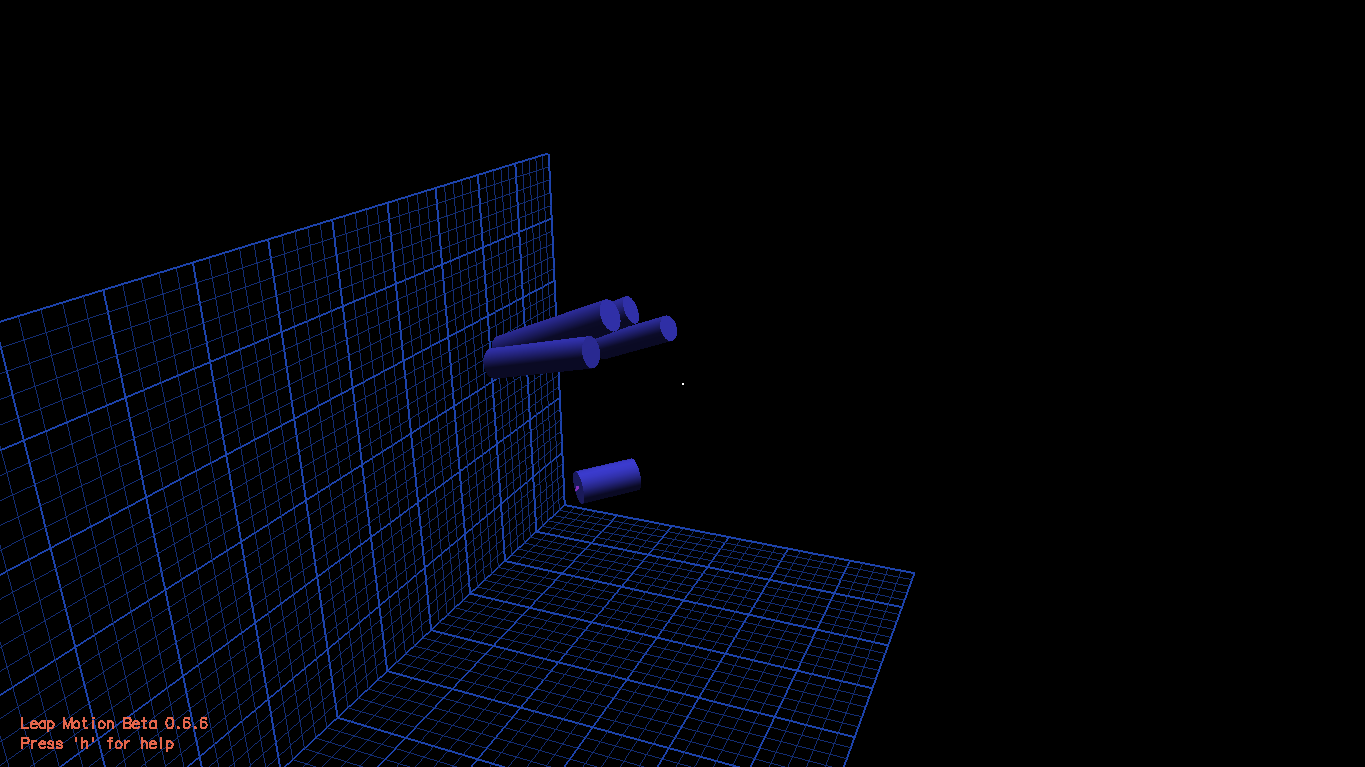
\includegraphics[width=\columnwidth]{images/hand-1.PNG}
    \caption{put our image about leap motion}
    \label{fig:teaser}
}

% Paper metadata (use plain text, for PDF inclusion and later re-using, if desired)
    \def\plaintitle{Handwriting in the air, Recognizing on the fly}
    \def\plainauthor{Sharad Vikram}
    \def\plainkeywords{handwriting recognition, time series, dynamic time warping}
    \def\plaingeneralterms{}

    \hypersetup{
        % Your metadata go here
            pdftitle={\plaintitle},
            pdfauthor={\plainauthor},  
            pdfkeywords={\plainkeywords},
            pdfsubject={\plaingeneralterms},
            % Quick access to color overriding:
                citecolor=black,
            linkcolor=blue,
            menucolor=black,
            urlcolor=blue,
    }

\usepackage{graphicx}   % for EPS use the graphics package instead
\usepackage{balance}    % useful for balancing the last columns
\usepackage{bibspacing} % save vertical space in references



\begin{document}

\maketitle

\begin{abstract}
Recent technologies in vision sensors are capable of capturing 3D finger positions and movements.
We propose a novel way to control and interact with computers by moving fingers in the air. The positions of fingers are precisely captured by a computer vision device. By tracking the moving patterns of fingers, we can then recognize users' intended control commands or input information.  We demonstrate this human input approach through an example application of handwriting recognition.
By treating the input as a time series of 3D positions, we propose a fast algorithm using dynamic time warping to recognize characters in online fashion. We employ various optimization techniques to recognize in real time as one writes. Experiments show promising recognition performance and speed.  

\end{abstract}

\keywords{\plainkeywords}
%\textcolor{red}{Mandatory section to be included in your final version.}

\category{H.5.2}{User Interfaces}{Input devices and strategies (e.g., mouse, touchscreen)}. 
%See \cite{ACMCCS} 
%See: \url{http://www.acm.org/about/class/1998/} 
%\textcolor{red}{Mandatory section to be included in your final version.}

%\terms{\plaingeneralterms}
%\textcolor{red}{Optional section to be included in your final version.}


% =============================================================================
\section{Introduction}
Interaction with computers can go far beyond typing on the keyboard,
moving the mouse, and touching the screen. 
Recent advances in computer vision technology can recognize 
hand gestures and body shape, as seen in Kinect games. 
With new computer vision devices such as the Leap Motion controller (), 
 precise 3D finger data can be obtained at over 100 frames per second.   
Therefore, it is possible to track the detailed positions of 
each finger precisely and efficiently. 
We advocate a new way to control computers by interpreting finger
movements as commands or character input using finger tracking devices.
In this paper, we propose a novel method to recognize handwritten
 characters in the air using such devices. 

\marginpar{
\begin{figure}
  \begin{center}
  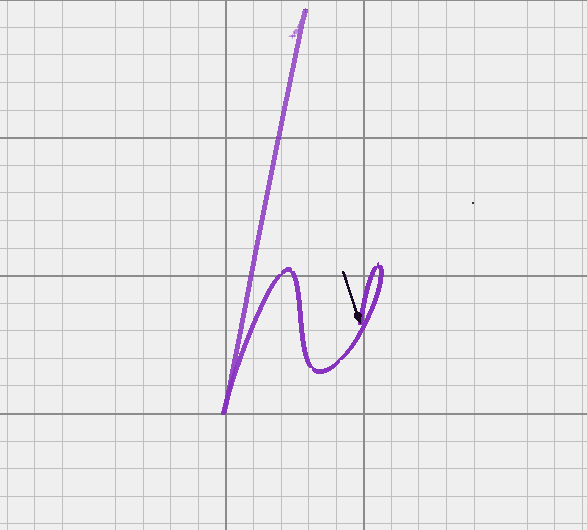
\includegraphics[width=1.75in]{images/he-2d-white-cropped.PNG}
  \caption{A 2D view of ``he'' sequence captured by Leap Motion controller.}
  \label{fig:he}
  \end{center}  
\end{figure}
}

Traditional character recognition technology is widely applied to such problems
as converting scanned books to text and converting images of bank checks into
valid payments. These problems can be divided into offline and online
recognition. 

We introduce a new problem: the online recognition of characters in a
 stream of 3D points from finger gestures. 
 Many OCR techniques utilize images of completed words, 
 whereas this paper deals with interpreting the data while it is generated,
specifically for the scenario of writing "in the air."  
In this paper we proposes a method of online character recognition, 
using a data-driven approach. 
Our method utilizes similarity search
technique on multi-dimensional time series. Figure~\ref{fig:he} shows a sample
sequences of 3D positions transformed from the tracked finger movement data. Our proposed approach to identify characters in these time series
 exploits the dynamic time warping (DTW) algorithm. 
A series of recent optimizations make a
DTW similarity search feasible in real time. This paper benchmarks the
performance of such a similarity search with the given application of
handwriting recognition.



The task of identifying characters in a time series requires data to test and
train on. Therefore, a new dataset needs to be created, partitioned into
 multiple candidate time series, specifically the characters in the alphabet,
  and multiple testing time series, which are words to be recognized. 
To construct this dataset, the Leap Motion, a commercial computer vision device,
is used to record data. The experiment will consist of collecting the same data
from over 100 people to account for differences in handwriting.

Our approach aims to deal with a less restricted kind of input than current
recognition techniques require. Related work shows that much of modern
handwriting recognition relies on a pen up/pen down gesture to 
The difference between our approach and other current handwriting recognition
approaches is the medium in which writing takes place. In many handwriting
recognition scenarios, the writing has already taken place and is being
statically analyzed. 
In our approach, we are dealing with live, free form input. 
Other related work shows the necessity of some pen up/pen down gesture 
to determine the beginning and end of meaningful input. 
Our approach attempts gives a less restricted form of input, 
where no strict gesture is necessary to identify meaningful data.



\section{Related Work}
Existing online handwriting recognition techniques depend on a pen up/pen down gesture to window the input data. Essentially, there is a known beginning and end to user input. This is not the case with this paper. We are using an input device that constantly streams the location of the fingers within its field of view so this type of gesture is not as easily done. Another technique used is the segmentation of the data points. This is difficult as it is hard to determine the end and beginning of segments, so typically unsupervised learning and data-driven approaches are used.[survey] The statistical approaches to this problem use Hidden Markov Models or use a combination of HMMs and neural networks to recognize characters~\cite{plotz2009markov}. Hilbert Warping has been proposed as an alignment method for handwriting recognition~\cite{ishida2010hilbert}. [hilbert] Other scenarios have been proposed, including one where an LED pen is tracked in the air. This allows for 3D data to be interpreted, but also allows for the beginning and end of input to be clearly defined.[katakana] Finally, treating the handwriting problem like speech recognition, ie treating the input points as a signal, allows in place algorithms with handwriting feature vectors to be used, but the same problem of segmentation arises.[speech] They also have problems with accuracy in identification. 
Another area of application of these techniques is sketch recognition, or digitizing drawings. The methods typically involve searching for sketch primitives and then combining them, but also rely on pen up/pen down gestures. [recognizing]


\section{Proposed approach}
\input{030proposed.tex}

\section{Experiments}
There are two parts to the dataset to be collected.

The first is "candidate" time series. The candidates consist of the letters of the alphabet, written in both uppercase and lowercase. Each letter will be replicated five times, for a total of 260 recordings per person. Around 100 people will participate in the instrument for a total of 26000 recordings.

The second part is "data" time series. The data time series are words to be tested. These words will be taken from Lincoln's Gettsyburg Address: "Four score and seven years ago our fathers brought forth on this continent, a new nation, conceived in Liberty, and dedicated to the proposition that all men are created equal." Each word will be recorded individually. This will also be replicated by 100 people, for a total of 30000 recordings.

Thus, the total size of the dataset will be 56000.

The data will be recorded with the LEAP Motion, using a browser application. \\
\begin{figure}
  \begin{center}
  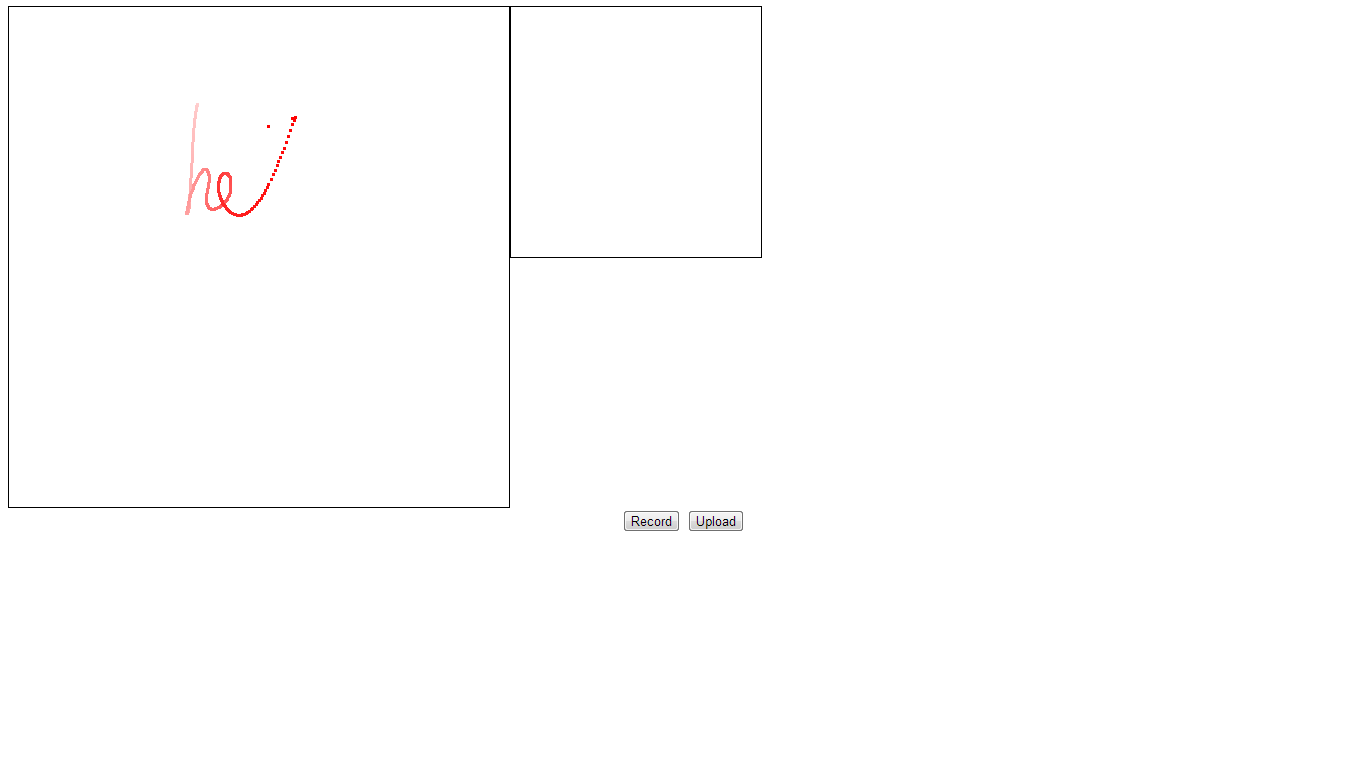
\includegraphics[width=\columnwidth]{images/recording-1.PNG}
  \caption{The data recording apparatus}
  \label{fig:teaser}
  \end{center}  
\end{figure}
The browser application shows a 2D preview of the data being recorded and prompts users to confirm the character or word they just wrote.
After the user has finished recording, the data will be uploaded, so at this stage, the user requires an internet connection.


\section{Conclusion and future work}
\input{050conclusion.tex}



\balance
\bibliographystyle{acm-sigchi}
\bibliography{BIB/leiliref}

\end{document}
